\documentclass[11pt, oneside]{article}
\usepackage[margin=1in]{geometry}
\geometry{letterpaper}
\usepackage{booktabs}
\usepackage{hyperref}
\usepackage{enumitem}
\usepackage{float}
\usepackage{caption}
\usepackage{subcaption}
\usepackage[numbers]{natbib}
\usepackage{graphicx}
\usepackage{amssymb}
\usepackage{amsmath}
\usepackage{array}
\usepackage{longtable}
\usepackage{xcolor}
\usepackage{tabularx}
\usepackage{setspace}
\usepackage{tikz}
\usetikzlibrary{positioning,arrows.meta,fit}
\hypersetup{
    colorlinks=true,
    linkcolor=blue,
    citecolor=blue,
    urlcolor=blue
}
\captionsetup{font=small,skip=3pt}
\setlength{\textfloatsep}{8pt}
\setlength{\floatsep}{6pt}
\setlength{\intextsep}{6pt}
\emergencystretch=2em
% ============================================================
% TITLE BLOCK --- students must keep this format
% Filename of the compiled PDF must be:
% CS781-CP-[Firstname]-[Lastname]-[RollNo]-report.pdf
% ============================================================
\title{CS781 Capstone Project:\\
In-House Legal Intelligence System}
\author{
    Nithin T M  \\
    230709 \\
    {\tt nithintm23@iitk.ac.in}\\
    Indian Institute of Technology Kanpur (IIT Kanpur)
}
\date{}
\begin{document}
\maketitle
\begin{abstract}
A law firm that cannot send client documents to an external service needs its own
language models. We build a seven-phase Indian legal NLP stack under that constraint, with
no pretrained weights and no external APIs. Phase~1 pretrains four 126M--151M-parameter
transformers from scratch (a GQA decoder, an encoder--decoder, a latent-attention decoder and
a pointer-generator decoder) on 1.255B tokens of Supreme Court, High Court, tribunal and
statute text with our own byte-level BPE. Phases 2--7 adapt these trunks with full
fine-tuning, eight parameter-efficient methods and distillation to NER, rhetorical roles,
judgment prediction, statute identification, summarization and prior-case retrieval. Three
findings recur. The four architectures are equivalent at iso-compute, and Phase-1 likelihood
does not predict downstream rank. Labelled data, not architecture or adaptation method, is
the binding constraint. Combining systems, and reading structure the data already carries,
moved the score more than any single model: we rank first in Phases 1 and 6 and second in Phases 4 and 7.
\end{abstract}

% ============================================================
\section{Competition Result}
% ============================================================
\noindent
\textbf{Codabench username:} \texttt{n\_230709}
\hfill
\textbf{Roll number:} 230709\\
\textbf{Code repository:} \url{https://github.com/FrankyWish/CS781-Capstone-Legal-NLP}
\medskip

\noindent
Table~\ref{tab:leaderboard} gives the entry shown on each leaderboard. Several are hybrids (lexical
models, rules or a Phase-1 corpus lookup), so the best Phase-1-model-only score is given beside it.

\begin{table}[H]
\centering
\small
\caption{Official phase scores and ranks (test). ``Model-only'' uses nothing but fine-tuned Phase-1 models.
$^{\dagger}$Trained with 5 additional labelled IL-TUR \texttt{rr} documents (Sec.~4.4).}
\label{tab:leaderboard}
\setlength{\tabcolsep}{3.5pt}
\begin{tabular}{clcccc}
\toprule
Phase & Task & Primary metric (value) & Model-only & Rank & Valid submissions \\
\midrule
1 & Legal LM pretraining & BERTScore F1 0.8689 & 0.8449 & 1 & 27 \\
2 & Legal NER & strict Macro-F1 0.6515 & 0.4873 & 7 & 65 \\
3 & Rhetorical role prediction & Macro-F1 0.6707$^{\dagger}$ & 0.5637 & 4 & 92 \\
4 & Court judgment prediction & Macro-F1 0.8767 & 0.7225 & 2 & 49 \\
5 & Legal statute identification & Macro-F1 0.4632 & 0.3949 & 6 & 62 \\
6 & Abstractive summarization & BERTScore F1 0.8606 & 0.8391 & 1 & 57 \\
7 & Prior case retrieval & Micro-F1@7 0.5157 & 0.3325 & 2 & 79 \\
\bottomrule
\end{tabular}
\end{table}
\noindent
\textbf{Total valid Codabench submissions across all phases:} 431\\
\textbf{Date ranks were recorded:} 9 November 2026, from each phase's leaderboard.
\medskip

Every phase exceeded the required minimum of distinct submissions. Phases 3--7 include the
compulsory LoRMA and knowledge-distillation runs among their counted submissions; in Phase~2 the
distillation run was submitted and the LoRMA run was evaluated by cross-validation.

% ============================================================
\section{Introduction and Problem Description}
% ============================================================
Indian court judgments are long and citation-heavy, and law firms processing them often can't send
the text to external APIs for confidentiality reasons. The constraint is that the whole stack has to
be trained and run within those bounds. Phase~1 needs 50M--300M parameters, trained from scratch on
the provided corpus only, and there have to be four architecturally distinct models. All later
phases start from one of those four---no external pretrained weights.

The phases cover generation (Phase~1), NER (Phase~2), rhetorical role classification (Phase~3),
outcome prediction (Phase~4), statute prediction (Phase~5), summarization (Phase~6), and prior case
retrieval (Phase~7). Phase~1: given 512 words, predict the next 128; 1000 test prompts, main metric
BERTScore F1~\citep{zhang2020bertscore}, secondary ROUGE-L and BLEU~\citep{lin2004rouge,papineni2002bleu}.
Phase~2: 12 entity types as exact character spans, strict Macro-F1. Phase~3: 13 rhetorical roles per
sentence, Macro-F1. Phase~4: allow/dismiss prediction on the judgment with the order removed, binary
Macro-F1. Phase~5: applicable statutes from 100 IPC/CrPC sections, Macro-F1. Phase~6: summarization,
BERTScore F1 with ROUGE-1/L secondary. Phase~7: return 7 cited prior cases per query judgment,
Micro-F1@7.

We compared Phase-1 likelihoods against downstream performance and tested parameter-efficient
adaptation against full finetuning across the smaller labeled sets. Many judgments are 5--30$\times$
longer than the context window, so we also tested truncation rules, retrieval, and hybrid
combinations. Hybrid systems with different training setups are reported separately; for model-only
evaluation we didn't consult public test labels.

% ============================================================
\section{Data Analysis and Preprocessing}
% ============================================================
\subsection{Sources and official splits}
All task data from \texttt{Exploration-Lab/CS-781-Capstone} and its official phase configs. Several
phases use public IL-TUR tasks~\citep{joshi2024iltur}: Phase~3 is IL-TUR \texttt{rr}~\citep{malik2022rr},
Phase~4 is CJPE from ILDC~\citep{malik2021ildc}, Phase~5 is \texttt{lsi}~\citep{paul2022lesicin},
Phase~6 is IN-Abs~\citep{shukla2022summ}, Phase~7 is IL-PCR~\citep{joshi2023ilpcr}. Split sizes and the
stats that most affected each phase's design are in Table~\ref{tab:data}.

\begin{table}[t]
\centering
\scriptsize
\caption{Split sizes and the measured statistics that shaped each phase.}
\label{tab:data}
\begin{tabular}{@{}c>{\raggedright\arraybackslash}p{3.3cm}>{\raggedright\arraybackslash}p{9.6cm}@{}}
\toprule
Phase & Train / dev / test & Statistic and consequence \\
\midrule
1 & 1.255B tokens (SC 254.7M, HC 450.0M, tribunals 400.0M, Acts 150.0M) / 500 windows / 1{,}000 & A source classifier (86.5\% held-out accuracy) puts 87\% of test prompts in the Supreme Court source $\Rightarrow$ SC-annealed data mix. 32\% of 60 probed test prompts occur verbatim in the corpus $\Rightarrow$ retrieval (Sec.~\ref{sec:p1}). \\
2 & 70 docs, 8{,}393 entities (2 folds) / -- / 35 & Median document 26{,}640 characters, 7--28$\times$ the window; labels range from 184 (R.COUNSEL) to 1{,}575 (DATE); 98.33\% of spans survive char$\to$token$\to$char; 67.4\% of entity strings repeat inside their document. \\
3 & 90 docs, 18{,}987 sentences / -- / 10 docs & 496 sentences repeat in train/dev and their labels agree only 77.1\% of the time; PrecedentOverruled has 3 sentences, Dissent occurs in 2 orders and in no test document. \\
4 & 32{,}305 unique / 994 / 1{,}517 & 41\% positive in train, 50\% in dev; median 2{,}534 BPE tokens, 30\% over 4{,}096; all 1{,}517 test texts had labelled copies in the first \texttt{dev.json} (dropped, reported). \\
5 & 42{,}750 / 10{,}053 / 13{,}019 & 100 statutes, each with $\geq$50 train documents; facts are masked (\texttt{<SECTION>}, \texttt{<ACT>}), only 2.9--4.1\% keep a section number; median 637 tokens. \\
6 & 7{,}028 / 600 held out / 100 & Document 3{,}147 words, summary 642 (medians); summary 8-gram copy rate 0.32; BERTScore saturates at $\approx$450 words. \\
7 & 827 q / 118 q / 237 q; pools 4{,}320 / 1{,}023 / 1{,}727 & 6.42 golds per train query (max 92 in dev); dev ceiling Micro-F1@7 0.6181; median 5{,}750 query tokens; every test query is in its own pool. \\
\bottomrule
\end{tabular}
\end{table}

\subsection{Corpus statistics that actually informed design}
\label{sec:stats}
\textbf{Phase~1.} Dropped documents under 900 words---anything shorter doesn't fill a 1024-token
window even with random-offset sampling, and the High Court subcorpus in particular has a lot of short
case header records mixed in. Mean lengths: Acts 6138 words, Supreme Court 3722, tribunals 1435, High
Courts 941 (from random-offset sampling). The SC corpus has only 254.7M tokens, so training used three
mixing stages: first 60\% of steps at 35/30/25/10\% (SC/HC/tribunal/Acts), next stage to 90\% at
70/20/10/0\%, final 10\% SC only with lr decaying to zero.
\textbf{Phase~2.} $\sim$95\% of tokens are outside any entity; we used inverse frequency weights raised
to 0.5 to address the imbalance.
\textbf{Phase~4.} Outcome phrases present in the last 1500 chars of a small fraction of documents in
every split, so order removal isn't complete.
\textbf{Phase~6.} BERTScore compares at most 512 RoBERTa-large tokens per side. A 450-word prefix of a
reference scores 1.000 against the full reference; ROUGE-1 of the same prefix is only 0.609. With median
reference length 642 words, only roughly the first 420 words of a generated summary affect this metric.
\textbf{Phase~7.} Candidate pools come from citations inside the query judgments. Year-based filtering
would have removed 23\% of dev gold cases, so we did not apply it.

\subsection{Preprocessing}
\label{sec:prep}
\textbf{Tokenization.} Byte-level BPE, 32768 vocab, extending the course A-1 implementation.
Pre-tokenizer splits digit runs of at most 3 and detaches punctuation---\emph{Act}, \emph{Act,} and
\emph{Act.} map to the same type. On a 20MB test sample this cut distinct chunk types from 115852 to
52515. No lowercasing or Unicode normalization; decoding is exactly invertible with zero failures on
100 documents.

\textbf{Character offsets for NER.} Byte-level BPE can split multi-byte Devanagari characters across
tokens, so each byte is mapped to its enclosing character instead of enforcing character boundaries on
tokens. The pre-tokenizer prepends a space to each word, which caused a gold span $(7, 29)$ to decode as
$(6, 29)$; trimming whitespace in decoding fixes this.

\textbf{Sentences and long documents.} Phase~3 uses the provided sentence lists. Sentences over 128
tokens (2.3\%) keep head and tail. Phase~4 reads multiple 512-token chunks spread across the judgment.
Phase~5 truncates at 8192 tokens, 3/4 from front, 1/4 from tail. Phase~6 gives neural models
head-70\%/tail-30\% of a 1152--2048 token budget or selected sentences. Phase~7 encodes with 8 chunks of
1024 tokens, scores via max chunk similarity. All phases remove copies of test documents from train and
dev using normalized text or rare $n$-grams.

% ============================================================
\section{Approach and Model Evolution}
% ============================================================
\subsection{Phase-1 foundation model}
\label{sec:p1}
All four models: $d_{\text{model}} = 768$, 12 attention heads (dim 64), SwiGLU FFN~\citep{shazeer2020glu}
hidden size 2048, RMSNorm~\citep{zhang2019rmsnorm}, RoPE~\citep{su2021roformer}, 1024-token context,
tied embeddings.

\textbf{M1} (\texttt{LexArc-D}, 125.9M): 16-layer decoder, grouped-query attention~\citep{ainslie2023gqa},
12 query heads sharing 4 KV heads. \textbf{M2} (\texttt{LexArc-ED}, 151.0M): 10-layer bidirectional
encoder, 8-layer decoder; seq2seq loss gives the encoder no direct gradient, so it trains with
$\mathcal{L} = \mathrm{CE}_{\text{dec}} + 0.3\,\mathrm{CE}_{\text{MLM}}$ and 15\% masked tokens.
\textbf{M3} (\texttt{LexArc-L}, 129.0M): replaces GQA with multi-head latent
attention~\citep{deepseek2024v2}, latent width 256, same KV-cache width as M1, RMSNorm on the latent,
RoPE on queries and reconstructed keys. \textbf{M4} (\texttt{LexArc-P}, 126.0M): M1 plus a
pointer-generator head~\citep{see2017pointer}:
\[
p(y) = g\,p_{\text{vocab}}(y) + (1-g)\sum_{j \le t,\; x_j = y} a_{tj}
\]
We ran an early test where adding an untrained copy bias toward prompt tokens gave $+0.0028$ BERTScore
on M1 and $+0.0025$ on M2---this motivated the pointer head. Computed in log space with
\texttt{logsumexp}; the probability-space version got NaN after 700 steps because the derivative of
$\log(x + 10^{-9})$ at $x=0$ is very large.

Three shared modifications, controlled by config flags: value residual~\citep{zhou2024value}, QK-norm
with $10^{-4}$ z-loss~\citep{dehghani2023vit22b}, 4 register tokens~\citep{darcet2024registers}.
Optimizer: Muon~\citep{jordan2024muon} lr 0.025 on 2D hidden weights, AdamW lr $10^{-3}$ wd 0.1 on
embeddings/norms/head. 2\% warmup, cosine schedule by wall time, batch $24\times1024$ tokens, bf16,
\texttt{torch.compile}, 6hr budget (586M--680M tokens). Parameter counts verified before training and
again on built modules.

Sanity checks before the main runs: input-target shift, single-batch overfit, KV-cache output vs full
forward pass. 34M ablation (40M tokens, one change per run): Muon vs AdamW $-0.486$ val loss, QK-norm +
z-loss $-0.259$, value residual $-0.024$, registers $+0.022$. Registers hurt in the ablation; kept them
in all main models to hold configuration constant.

Decoding: temp 0.8, top-$p$ 0.95, rep penalty 1.05, no-repeat 4-grams, prompt-copy logit bias 2--3 for
M1 and M3 (M4 has the pointer head instead). Settings chosen per model on dev with bootstrap intervals.
Every continuation padded to 128 words. Final generator uses MBR~\citep{kumar2004mbr} over 18 candidates
(6 each from M1, M3, M4), BERTScore as utility. Aho--Corasick automaton~\citep{aho1975efficient} over
last 20 words of each prompt flags corpus-found prompts; for those 308/1000 prompts the following 128
source words replace the generated text. M1 then got 4 more hours on SC text at the full learning rate;
\texttt{M1\_SC} is 0.104 nats better on held-out SC text and is the default trunk for downstream phases.

\subsection{Transfer protocol (Phases 2--7)}
All later phases initialize from Phase-1 checkpoints and add a task head. Lexical models in hybrids are
the only things trained from scratch. Figure~\ref{fig:system} shows the full stack. Decoders run
causally unless noted; M2 contributes its encoder.

Adaptation methods, all implemented directly without the \texttt{peft} library: full finetuning;
LoRA~\citep{hu2022lora} and rsLoRA~\citep{kalajdzievski2023rslora}; LoRMA~\citep{bihany2025lorma}---the
multiplicative variant $h = (I + \tfrac{\alpha}{r}BA)\,W_0 x$, evaluated as $y = W_0x$,
$y + \tfrac{\alpha}{r}B(Ay)$, with rank inflation that recovers the pretrained function at
initialization; QLoRA~\citep{dettmers2023qlora} NF4 with double quantization;
AdaLoRA~\citep{zhang2023adalora}; Houlsby~\citep{houlsby2019adapters} and
Pfeiffer~\citep{pfeiffer2021adapterfusion} adapters; IA$^3$~\citep{liu2022ia3}; prefix
tuning~\citep{li2021prefix}; BitFit~\citep{benzaken2022bitfit} adapted for RMSNorm gains and added
biases; layer-wise lr decay with partial finetuning; gradual unfreezing~\citep{howard2018ulmfit}.

Knowledge distillation: every other layer of the teacher kept, layer 0 always retained since the value
residual reads it; trains on $\alpha T^2\,\mathrm{KL}(p_s \,\|\, p_t) + (1-\alpha)\,\mathrm{CE}$~\citep{hinton2015distilling,sanh2019distilbert}.

\begin{figure}[t]
\centering
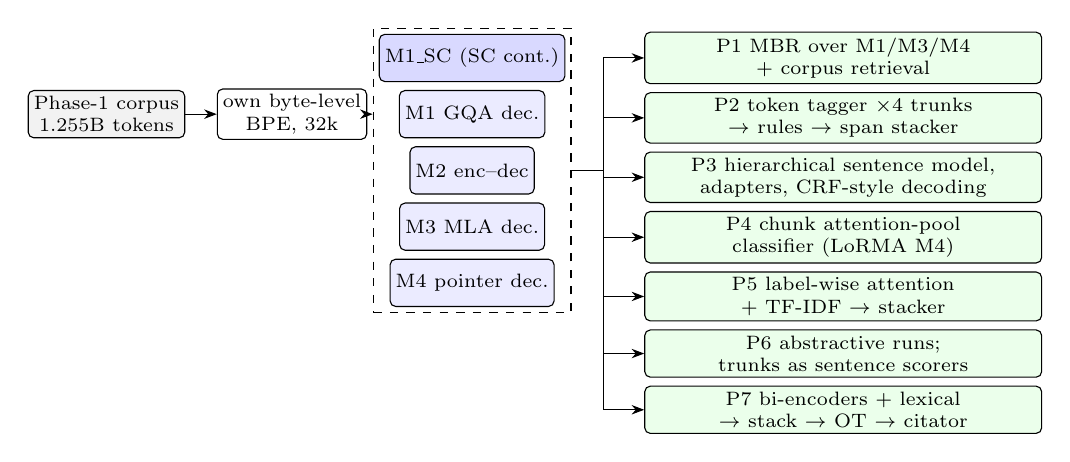
\begin{tikzpicture}[font=\scriptsize, node distance=3mm and 4mm,
  box/.style={draw, rounded corners=2pt, align=center, inner sep=2pt, minimum height=6mm},
  arr/.style={-{Stealth[length=1.6mm]}}]
\node[box, fill=gray!10] (corpus) {Phase-1 corpus\\1.255B tokens};
\node[box, right=of corpus] (bpe) {own byte-level\\BPE, 32k};
\node[box, right=of bpe, fill=blue!8] (m1) {M1 GQA dec.};
\node[box, below=1mm of m1, fill=blue!8] (m2) {M2 enc--dec};
\node[box, below=1mm of m2, fill=blue!8] (m3) {M3 MLA dec.};
\node[box, below=1mm of m3, fill=blue!8] (m4) {M4 pointer dec.};
\node[box, above=1mm of m1, fill=blue!15] (m1sc) {M1\_SC (SC cont.)};
\node[draw, dashed, fit=(m1sc)(m4), inner sep=2pt] (trunks) {};
\node[box, right=10mm of m1sc, fill=green!8, text width=4.9cm] (p1) {P1 MBR over M1/M3/M4 + corpus retrieval};
\node[box, below=1mm of p1, fill=green!8, text width=4.9cm] (p2) {P2 token tagger $\times$4 trunks $\to$ rules $\to$ span stacker};
\node[box, below=1mm of p2, fill=green!8, text width=4.9cm] (p3) {P3 hierarchical sentence model, adapters, CRF-style decoding};
\node[box, below=1mm of p3, fill=green!8, text width=4.9cm] (p4) {P4 chunk attention-pool classifier (LoRMA M4)};
\node[box, below=1mm of p4, fill=green!8, text width=4.9cm] (p5) {P5 label-wise attention + TF-IDF $\to$ stacker};
\node[box, below=1mm of p5, fill=green!8, text width=4.9cm] (p6) {P6 abstractive runs; trunks as sentence scorers};
\node[box, below=1mm of p6, fill=green!8, text width=4.9cm] (p7) {P7 bi-encoders + lexical $\to$ stack $\to$ OT $\to$ citator};
\draw[arr] (corpus) -- (bpe); \draw[arr] (bpe) -- (trunks.west |- bpe);
\draw[arr] (trunks.east) -- ++(4mm,0) |- (p1.west);
\foreach \p in {p2,p3,p4,p5,p6,p7} \draw[arr] (trunks.east) ++(4mm,0) |- (\p.west);
\end{tikzpicture}
\caption{One corpus and tokenizer, four Phase-1 trunks (plus the SC-continued M1), and seven
separately fine-tuned task systems. No phase feeds its predictions into another.}
\label{fig:system}
\end{figure}

\subsection{Phase 2 - Legal NER}
BIO token classification, character offsets recovered as in Sec.~\ref{sec:prep}. Documents chunked into
1024-token windows, spans merged across windows. Best single model: M4 at 0.329 CV vs 0.294 for
\texttt{M1\_SC}.

Strict F1 on CV was 0.30 vs overlap F1 0.58. The oracle---string-matching gold forms per
document---scores 0.9863, so the gap is in boundary precision, not detection.

Final system: (i)~\textbf{Members.} Full finetunes of all 4 trunks, log-prob averaged, three data
variants: gold only; gold + rule-labeled corpus text; gold + InLegalNER~\citep{kalamkar2022ner} with 11
test-leaking records removed. (ii)~\textbf{Postprocessing.} Spans expanded to whole words (except
PREC---6.76\% of gold spans end mid-token). Each span replaced by the longest same-label prediction
containing it. 26 regex rules checked on all 8393 gold spans; 6 failed and were dropped.
(iii)~\textbf{Stacker.} Gradient-boosted classifier~\citep{ke2017lightgbm} trained over every candidate
span from 3 systems at 3 postprocessing stages, features: agreement counts, in-document repetition,
shape. Cross-fitted on CV predictions, selected on the worse fold; threshold emits 136 spans/doc.
(iv)~\textbf{Final correction.} Precision trim: keep a span only if another stack also emits it
exactly. Recall rounds add spans where two systems agree.

\subsection{Phase 3 - Rhetorical role prediction}
Phase-1 trunk encodes packed sentence chunks up to 512 tokens. Each sentence mean-pooled; 2-layer
transformer over all document sentences with position and domain features. Training: windows of 64
sentences.

Decoding: prior correction $\tau$ and label transition score $\beta$ as a linear-chain
CRF~\citep{lafferty2001crf}. Both legal domains trained jointly with a domain feature. 5-fold document CV
over 90 documents; submission averages five fold model logits on test.

External coarse labels from MARRO~\citep{bhattacharya2019rr}, Kalamkar et al~\citep{kalamkar2022rr},
LegalSeg~\citep{nigam2025legalseg} trained as allowed sets, loss $= -\log \sum_{y \in S} p(y)$. Best
model-only result: intermediate pass over 7117 LegalSeg judgments before LoRA on M4. Best overall
systems ensemble these with TF-IDF logistic regression.

One run added 5 additional labelled IL-TUR \texttt{rr} documents to training. Graded entry
\texttt{v68} (0.6707): LoRA on LegalSeg-pretrained M4 with 5 additional Income Tax documents in
training, ensembled with TF-IDF trained the same way. The model-only (0.5637) and hybrid (0.5879)
results, trained without these documents, are the fairer comparison between methods.

\subsection{Phase 4 - Court judgment prediction}
Trunk: M4 with LoRMA, rank 16 on $q$ and $v$. Reads $k$ chunks of 512 tokens bidirectionally,
mean-pools each chunk, attention pool with position-decile embeddings feeds a linear head. $k=4$ during
training, $k=8$ at test time ($+0.011$ dev). Trained on all gold cases + 14337 silver cases labeled from
corpus final orders (92.3\% agreement with gold on corpus copies of training cases; judgments matching
dev or test excluded).

Threshold tuned on 994 real dev cases. Phase-2/3 outputs not used as features. Graded entry includes a
lookup: 1345/1517 test judgments appear in the Phase-1 SC corpus, where text after the CJPE truncation
point is the removed order; 99.3\% accurate on dev where it fires.

\subsection{Phase 5 - Legal statute identification}
Neural head: one learned query per statute attending over trunk token states, 100 independent sigmoids,
binary cross-entropy.

Lexical members: TF-IDF word $n$-grams, one-vs-rest logistic regression, cross-fitted on dev (each dev
doc scored by a model trained on train + other three dev folds). Second-stage gradient-boosted stacker
over (doc, candidate) pairs for each doc's top 25--35 candidates: member z-scores, ranks, agreement,
label frequency, co-occurrence $P(j\mid k)\,p(k)$.

Thresholds: global or per-statute values shrunk toward it,
\[
t_\ell = \frac{n_\ell\, t_\ell^{*} + s\, t_{\text{glob}}}{n_\ell + s}, \qquad s = 25.
\]
2-fold CV on dev for threshold selection. Every doc gets at least one statute.

\subsection{Phase 6 - Abstractive summarization}
Abstractive members: decoder-only continuation for M1, M3, M4; encoder-decoder generation for M2, all
from Phase-1 inits. Documents truncated to head-70\%/tail-30\% of a 1152--2048 token budget or replaced
with selected sentences. Length targeted per document via regression on document features.

BERTScore reads only the first $\sim$420 words of each side (Sec.~\ref{sec:stats}), so we also ran an
extractive approach. \texttt{bsel} labels each training sentence by its marginal contribution under the
metric's token similarity tables (RoBERTa-large layer 17, for label construction only), then trains
gradient boosting on 27 sentence features. The extractive system outperformed the abstractive members.

\texttt{nsel} finetunes the top 4 blocks of each Phase-1 trunk to regress those sentence labels in
context, stacks the four trunk scores with \texttt{bsel}, emits top sentences in document order up to
target length. Only Phase-1 trunks and boosted trees at test time.

\subsection{Phase 7 - Prior Case Retrieval (PCR)}
Base ranking: TF-IDF (sqrt query weighting, $\text{max\_df}=0.2$) + BM25~\citep{robertson2009bm25} +
passage-level MaxP~\citep{dai2019maxp} + queries from text around each \texttt{CITATION} mask +
bi-encoders.

Bi-encoders share one encoder for queries and candidates (M2 encoder). 8 chunks of 1024 tokens, max
chunk similarity. Contrastive training~\citep{oord2018cpc} with in-batch + 3 hard negatives per method.

Gradient-boosted stacker combines all members with features normalized within each query. Test queries
ranked jointly with entropic optimal transport~\citep{cuturi2013sinkhorn}: 7 slots per query, candidate
column mass proportional to slot share, unbalanced relaxation fit on train only.

Header rules: some SC judgments retain judis metadata (\texttt{CITATION}, \texttt{DATE OF JUDGMENT},
\texttt{CITATOR INFO}). Candidate whose citator list contains the query's AIR key: dev precision 0.981.
Unmasked reporter citations in query body match candidate keys: 0.978. Candidates post-dating the query
demoted---352/352 consistent on dev. Phase-1 corpus lookup recovers masked case names, matched to
candidate titles: 0.905. Failed approaches in Sec.~\ref{sec:ablate}.

% ============================================================
\section{Experiments and Implementation Details}
% ============================================================
\subsection{Compute and training protocol}
Phase-1 models: 6 hours each + 4 hours per SC continuation. Task runs: 8--60 minutes; Phase~3 five-fold
$\sim$1.8 hours. Non-neural work (rules, stacking, retrieval, ensembling) on CPU from saved logits.

Checkpoints every 10--20 minutes, resume from \texttt{resume.pt}. Each driver skips already-finished
steps---the runtime was reset several times. Task finetuning: AdamW + cosine schedule, grad clip 1.0,
dropout 0.1 in task heads for Phases 2--6, bf16.

Model selection on held-out task metric (span-F1, Macro-F1, BERTScore, hits) rather than loss; best of
3--15 evals per run kept.

\begin{table}[t]
\centering
\scriptsize
\caption{Hyperparameters of the final neural component in each phase (adapter LR shown for PEFT runs).}
\label{tab:hparams}
\resizebox{\linewidth}{!}{%
\begin{tabular}{lccccccc}
\toprule
 & P1 & P2 & P3 & P4 & P5 & P6 & P7 \\
\midrule
Trunk / method & M1, M3, M4 & 4 trunks, full FT & M4, LoRA r16 & M4, LoRMA r16 & M1, adapters & M1--M4, top 4 blocks & M2 enc., LoRMA r8 \\
Parameters (M) & 125.9--129.0 & 125.9--151.0 & 126.0 & 126.6 (0.73 trained) & 125.9 & 125.9--151.0 & 151.3 \\
Context length & 1{,}024 & 1{,}024 & 512 / chunk & $8\times512$ & $6\times512$ & sentence window & $8\times1{,}024$ \\
Peak LR & 0.025 (Muon) / $10^{-3}$ & $3\times10^{-4}$ & $3\times10^{-4}$ & $3\times10^{-4}$ & method default & $5\times10^{-5}$ & $10^{-4}$ \\
Batch $\times$ accum. & $24\times1$ & $8\times1$ & 4 windows & 8 docs & 8 docs & 8 & 4 (+3 neg.) \\
Epochs / steps & 6 h wall-clock & 8 epochs & $\leq$15 epochs & 1 epoch & 1.5 epochs & 55 min & 600 steps \\
Dropout & 0 & 0.1 & 0.1 & 0.1 & 0.1 & 0.1 & 0 \\
Decoding / threshold & MBR $k{=}6$ + retrieval & 136 spans/doc & $\tau{=}0.25$, $\beta{=}0.25$ & dev-tuned & per-label, $s{=}25$ & length target & top 7 after OT \\
\bottomrule
\end{tabular}}
\end{table}

\subsection{Local evaluation}
Each phase made its own labeled held-out split from public data. Phase~1: 500 windows in test format,
random offsets, source proportions matched to test set, documents excluded from training by hash. Dev
BERTScore tracked test to within 0.002.

Phase~2: 2-fold CV on the organizers' folds, refitted on all 70 docs (test $\sim$1.23$\times$ CV).
Phase~3: 5-fold document CV. Phases 4 and 5: real dev docs with test copies removed. Phase~5 threshold
selection: 2-fold CV on dev. Phase~6: 600 held-out training docs, paired half-split, 2-SE bar. Phase~7:
118 dev queries, 1 hit = 0.00111 F1, paired 2-SE bar $\sim$11 hits.

Every submission zip re-scored with the official evaluators. Weak models lost 0.02--0.06 on test; strong
ones shifted under 0.015 (Phase~4). Phase~2 CV-to-test ratio fell 1.23 to 1.10 to 1.02 as data grew.
Phase~7 test sat $\sim$0.004 below dev at the top.

\subsection{Ablations and controlled comparisons}
\label{sec:ablate}
\textbf{Architecture and Phase-1 transfer.} At iso-compute, 0.8346--0.8386 on Phase-1 test---within
noise. Encoder-decoder lost 0.0096 (53\% of tokens have gradient). Phase-1 likelihood ranked decoders in
reverse order vs BERTScore and also mis-predicted downstream rank. M4 was best for Phases 2, 3, 4; its
copy channel makes likelihood a noisy signal for the trunk. Continuing SC pretraining at the full
learning rate beat 25\% lr on every in-domain measure ($-0.104$ vs $-0.067$ nats).

\textbf{Adaptation method, one factor at a time.} Same 10k Phase-4 docs: LoRMA 0.634 dev vs full
finetuning 0.610 at 0.6\% of the parameters and 30\% less memory. Phase~3: LoRA on M4 (0.522 test) beat
full finetuning of M4 with 3$\times$ the data (0.491). Phase~6: LoRMA and full finetuning tied at 0.8343.
Phase~7: LoRMA 0.352 dev, full finetuning 0.340, LoRA 0.331. Phase~2: LoRMA on M3 got 0.211 CV vs 0.285
for full finetuning---with only 70 training documents the trunk weights have to shift. Distillation: 88\%
(P2), 96\% (P4), 94\% (P7) of teacher performance at half depth, 1.9--2$\times$ throughput.

\textbf{Long documents.} 4 chunks spread across the judgment beat last 2 chunks by 0.018 dev on
Phase~4. TF-IDF over the whole judgment beat TF-IDF over the last 6000 chars by 0.032. Phase~6: selected
input sentences didn't help the neural model (0.8347 vs 0.8403 for plain truncation at equal prompt
length).

\textbf{Negative results.} BIOES, CRF, caption prepending, cross-document gazetteer, per-label source
arbitration---all failed in Phase~2. Stacking lost in Phase~3 (0.448 vs 0.464 OOF). Silver statute labels
(precision 0.58, recall 0.33) and a citation rule gave nothing in Phase~5. Neural + extractive hybrids
and neural openers before extraction lost to pure extraction in Phase~6. Zero-shot bidirectional use of a
causal decoder~\citep{behnamghader2024llm2vec} cost 50 dev hits in Phase~7; RM3~\citep{lavrenko2001rm}
query expansion was mostly noise.

% ============================================================
\section{Results}
% ============================================================
Table~\ref{tab:variants} lists the main variants with dev and test scores, model-only systems separated
from hybrids and lookups. Figure~\ref{fig:scaling} shows Phase-4 Macro-F1 vs training documents and
Phase-1 test score vs prompts served by retrieval. Scaling pretraining 10.6$\times$ (55M to 586M tokens)
moved test BERTScore from 0.8308 to 0.8359.

\begin{table}[t]
\centering
\scriptsize
\caption{Main variants per phase. Dev is held-out split (CV for P2, P3, P5); test is Codabench.
K: M = Phase-1 models only, H = hybrid with lexical models or rules, L = Phase-1 corpus lookup. A = trained with 5 additional IL-TUR \texttt{rr} documents. Bold = graded entry.}
\label{tab:variants}
\setlength{\tabcolsep}{3pt}
\begin{minipage}[t]{0.495\linewidth}\centering\resizebox{\linewidth}{!}{%
\begin{tabular}[t]{@{}clccc@{}}
\toprule
P & Variant & K & Dev & Test \\
\midrule
1 & M1, raw decoding & M & 0.8357 & 0.8359 \\
1 & M1, swept decoding & M & 0.8402 & 0.8384 \\
1 & M2 / M3 / M4, swept & M & 0.8306 / 0.8386 / 0.8350 & 0.8293 / 0.8386 / 0.8350 \\
1 & MBR, M1+M3+M4, 18 cand. & M & 0.8463 & 0.8449 \\
1 & + corpus retrieval (308) & L & -- & \textbf{0.8689} \\
\midrule
2 & M1\_SC, bidirectional & M & 0.294 & 0.3854 \\
2 & ensemble, 4 trunks, M4$\times$3 & M & 0.375 & 0.4608 \\
2 & + InLegalNER members & M & 0.477 & 0.4873 \\
2 & + snap, expansion, rules & H & -- & 0.5577 \\
2 & stacker, 3 systems $\times$ 3 stages & H & 0.616 & 0.6421 \\
2 & + trim and recall rounds & H & -- & \textbf{0.6515} \\
\midrule
3 & LoRMA M3 & M & 0.447 & 0.5045 \\
3 & rsLoRA M1 & M & 0.448 & 0.5193 \\
3 & LoRA M4 & M & 0.455 & 0.5223 \\
3 & full FT M4, + additional data & M & 0.473 & 0.4912 \\
3 & KD, 8-layer M4 student & M & -- & 0.5140 \\
3 & LoRA M4 after LegalSeg & M & 0.482 & 0.5637 \\
3 & 8-member ens.\ + TF-IDF (\texttt{v54}) & H & 0.491 & 0.5845 \\
3 & 3-member ens.\ (\texttt{v46}) & H & -- & 0.5879 \\
3 & + 5 IL-TUR \texttt{rr} docs (\texttt{v68}) & A & 0.493 & \textbf{0.6707} \\
\bottomrule
\end{tabular}}
\end{minipage}\hfill
\begin{minipage}[t]{0.495\linewidth}\centering\resizebox{\linewidth}{!}{%
\begin{tabular}[t]{@{}clccc@{}}
\toprule
P & Variant & K & Dev & Test \\
\midrule
4 & LoRMA / full FT / KD, 10k docs & M & 0.634 / 0.610 / 0.606 & 0.613 / 0.552 / 0.567 \\
4 & LoRMA, gold+silver, 8 chunks & M & 0.719 & 0.7080 \\
4 & 3 M4 runs averaged & M & 0.722 & 0.7225 \\
4 & + whole-judgment TF-IDF & H & 0.752 & 0.7488 \\
4 & corpus order lookup + M4 & L & 0.879 & \textbf{0.8767} \\
\midrule
5 & LoRMA M4 / adapters M1 & M & 0.347 / 0.363 & 0.3479 / 0.3610 \\
5 & QLoRA M3 / KD student & M & 0.359 / 0.344 & 0.3556 / 0.3464 \\
5 & neural ensemble & M & 0.395 & 0.3949 \\
5 & + TF-IDF & H & 0.424 & 0.4387 \\
5 & stacker, 8-seed bag & H & 0.459 & 0.4622 \\
5 & best single stacker seed & H & -- & \textbf{0.4632} \\
\midrule
6 & LoRMA M4 / full FT M4 & M & 0.8347 / 0.8345 & 0.8343 / 0.8343 \\
6 & KD, half-depth M1 & M & 0.8306 & 0.8277 \\
6 & reranker, abstractive cand. & M & 0.8425 & 0.8391 \\
6 & \texttt{bsel} extraction & H & 0.8549 & 0.8546 \\
6 & \texttt{nsel4}, 4 trunks as scorers & M+H & 0.8625 & \textbf{0.8606} \\
\midrule
7 & TF-IDF / zero-shot dense M2 & -- & 0.3769 / 0.3202 & 0.3757 / 0.3095 \\
7 & LoRMA bi-enc.\ / KD student & M & 0.3524 / 0.3313 & 0.3325 / 0.3154 \\
7 & stack, lexical + dense + MaxP & H & 0.4247 & 0.4241 \\
7 & + transductive OT decoding & H & 0.4636 & 0.4536 \\
7 & + citator rules & H & 0.5092 & 0.4979 \\
7 & + corpus lookup & L & 0.5147 & \textbf{0.5157} \\
\bottomrule
\end{tabular}}
\end{minipage}
\end{table}

\begin{figure}[t]
\centering
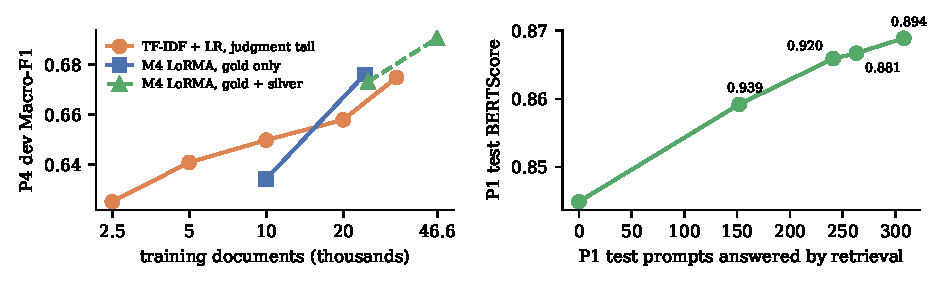
\includegraphics[width=0.8\linewidth]{figures/fig_scaling.pdf}
\caption{Left: Phase-4 dev Macro-F1 against training documents (log scale); silver cases are worth
about as much as gold ones. Right: Phase-1 test BERTScore as more prompts are answered by retrieval;
labels give the inferred quality of each newly retrieved batch.}
\label{fig:scaling}
\end{figure}

In Phase~1 all four architectures converged within 0.004; MBR and corpus retrieval gave larger gains
than architecture. Phase~2 models found entities but got boundaries wrong; the span stacker gave +0.057
test, more than any model change, by using different systems for different span types. In Phase~6
extractive selection with metric-derived labels beat the abstractive members by 0.0215 (the metric only
reads the first $\sim$420 words of each side, see Sec.~\ref{sec:stats}). In Phase~7 the citator headers
were essentially a direct citation-graph lookup.

% ============================================================
\section{Error Analysis and Discussion}
% ============================================================
\subsection{Phase-wise failure modes}
\textbf{Phase~1.} Greedy decoding had best function-word fluency but worst BERTScore ($-0.022$).
Repetition loops like ``the words used in the clause must be given a restricted meaning and that the
words used in the clause\ldots'' create bigrams that a fluency proxy rewards, hence the 4-gram repeat
limit. Citation-heavy continuations under-generate (36 words from 210 tokens). Shorter retrieval needles
pull in passages quoted inside other cases; quality dropped from 0.939 to 0.881 as needle length fell
from 40 to 20 words, approaching the 0.845 crossover.
\textbf{Phase~2.} Boundary errors: $\sim$38\% start, 41\% end, 21\% both. Biggest: truncations---\emph{ACHUTANANDA
PUROHIT} returned as \emph{CHUTANANDA PUR}. BIO merges adjacent same-label entities on bench lines. APP,
RESP, WIT, AUTH are predominantly missed detections and account for about a third of the metric. Final
system: recall 0.684 vs precision 0.625, only top-7 entry with recall clearly above precision.
\textbf{Phase~3.} Most common confusions: PrecedentReliedUpon vs Ratio (1215 sentences), Fact vs Ratio
(556), ArgumentRespondent vs ArgumentPetitioner (309). Two labels score zero across all submissions.
\textbf{Phase~4.} Weak models lost 0.02--0.06 from dev to test; TF-IDF lost 0.03.
\textbf{Phase~5.} After 0.56 epoch the four trunks are within 0.03 of each other. Per-label thresholds
overfit the rare statutes without heavy shrinkage ($s=25$).
\textbf{Phase~6.} The rank-1 system only leads on BERTScore. ROUGE-1 (0.580) and ROUGE-L (0.296) are
below several lower-ranked entries.
\textbf{Phase~7.} Of dev golds missed by the best system: 185 never retrieved, 164 in base top-20, 111
are rule matches bumped from queries with more than 7 rule-matched golds. Only 4 wrong rule matches make
top-7. Remaining errors are in the 45\% of queries with no header rule and no corpus copy.

\subsection{What the metrics do not measure}
BERTScore and ROUGE measure surface similarity to a reference. The rank-1 summarizer length was tuned to
the first $\sim$420 words BERTScore reads, so ROUGE scores are below several lower-ranked entries.
Span-F1 scores zero for a correctly typed entity with a one-character boundary offset. Many of the top
leaderboard numbers also reflect corpus access---test prompts, removed orders, headnotes, and citation
graphs are present in the permitted corpus or released text.

\subsection{Limitations and what you would do next}
6-hour training budget per model, 1024-token context, no human legal evaluation, phases trained
independently. Next steps: retrain without register tokens with document-boundary-aware packing; extend
context to 4096 with RoPE scaling; use Phase-3 Ratio/Ruling labels as features in Phases 4 and 6;
cross-fit neural Phase-5 members on dev; measure Phase-4 memorization on corpus-matched (901) vs
unmatched (93) dev cases.

\subsection{Surprising findings}
M4 had the best held-out next-token likelihood among the decoders but the worst Phase-1 BERTScore
(0.8350 vs 0.8386/0.8384 for M3/M1 from Table~\ref{tab:variants}). The pointer head may be causing the
model to copy more than is good for generation, inflating likelihood while hurting BERTScore---we didn't
investigate this further. M4 was still the strongest trunk for Phases 2, 3, and 4. Continuing SC
pretraining at the full learning rate beat the conventional reduced rate on every in-domain measure
($-0.104$ vs $-0.067$ nats), which runs against the standard advice. In Phase~7 the four strongest stacks
ranked in reversed order on test vs dev (Spearman $-1.0$); their dev differences were within the paired
2-SE interval.

% ============================================================
\section{Conclusion}
% ============================================================
All learned components in this stack came from four 126M--151M models trained from scratch in 6 hours
each. Span stacking in Phase~2, metric-derived sentence selection in Phase~6, and citator lookups in
Phase~7 each gave larger gains than changing model architecture or adaptation method. LoRMA was best in
Phases 4 and 7 and matched full finetuning in Phase~6; the adaptation method mattered more in Phase~2,
where only 70 training documents forced the trunk weights themselves to shift and full finetuning won.
Scaling pretraining had diminishing returns; the binding constraints were labeled data size and context
length.

% ============================================================
\clearpage
\section*{LLM Usage Declaration}
% ============================================================
\noindent
\textbf{Q1.} Which Large Language Model(s), if any, did you use while completing the competition or writing this report? \\[0.6em]
Answer: ChatGPT and Claude.

\medskip
\noindent
\textbf{Q2.} For each row, mark Yes or No and state the purpose in one short phrase.
\begin{table}[H]
\centering
\small
\begin{tabular}{>{\raggedright\arraybackslash}p{4.6cm}|c|>{\raggedright\arraybackslash}p{7.6cm}}
\toprule
Part & Used LLM? & Purpose of using the LLM \\
\midrule
Understanding concepts / papers & Yes & Clarifying technical concepts, methods and evaluation metrics \\
Ideation / brainstorming at a high level & Yes & Exploring possible experimental approaches and configurations \\
Debugging small ancillary snippets & Yes & Resolving minor implementation, environment and numerical issues \\
Plotting / visualization code & Yes & Assistance with plotting and figure formatting \\
Grammar / writing style of the report & Yes & Language refinement and editing \\
Report structure / section wording & Yes & Organising the report and improving section clarity \\
Designing the model architecture & Yes & Exploring architecture alternatives and implementation approaches \\
Hyperparameter search / tuning & Yes & Assistance with sweep scripts and candidate parameter ranges \\
Analysis of results / conclusions & Yes & Assistance in organising experimental observations and presenting results \\
Writing the core training / inference code & Yes & Implementation assistance for training, inference and pipeline components \\
Other (specify) & Yes & Assistance with submission validation, packaging and repository documentation \\
\bottomrule
\end{tabular}
\end{table}

\medskip
\noindent
\textbf{Q3.} Did you refer to sources other than lecture slides and an LLM? \\[0.4em]
Answer: \textbf{Yes.}

\noindent
I referred to the research papers listed in the bibliography, including works on LoRMA, LoRA, QLoRA,
AdaLoRA, adapters, knowledge distillation, MBR, pointer-generator networks, MLA, Muon and BERTScore, along
with the relevant dataset papers for IL-TUR, ILDC, IN-Abs and IL-PCR.

\noindent
I also used the official starter notebook and evaluation scripts, along with my previous CS781 assignment
implementations (A-1 BPE and A-3 Transformer) as a starting point for extending the tokenizer and model
modules. Additional datasets and research resources included InLegalNER, MARRO, Kalamkar et al.'s
rhetorical roles and LegalSeg.

\medskip
\noindent
\textbf{Q4.} Apart from any permitted LLM use, what was \emph{your} contribution?

\noindent
I independently drove the competition across all seven phases, from deciding the objectives and
experimental direction to selecting the final systems and submissions. I determined the scope of each
phase, identified the approaches worth exploring, designed the experimental comparisons and made the
decisions about which models to develop, retain, modify and submit.

\noindent
I handled the complete experimental execution on Google Colab, including selecting GPU configurations,
allocating and managing the available compute budget, scheduling training and inference runs, monitoring
their progress and recovering experiments when Colab runtimes were disconnected or recycled.

\noindent
After every experiment, I examined the resulting metrics and outputs, compared the different
configurations and used the observations to determine the next steps. For instance, I carried
\texttt{M1\_SC} forward from Phase~1 and subsequently moved towards M4 after the Phase~2 results showed
better fine-tuning behaviour. These decisions determined how the subsequent phases were developed.

\noindent
I worked on extending the existing tokenizer and Transformer implementations, developing the model
variants and task-specific components, integrating the different training and inference stages, and
adapting the pipelines to the competition's evaluation requirements. I also conducted the experiments,
handled implementation issues, investigated unexpected results and iteratively modified the systems based
on their observed performance.

\noindent
I was responsible for the experimental comparisons and the interpretation of the results across phases.
This included evaluating model-only and hybrid approaches, examining the contribution of additional
components, comparing performance across datasets and metrics, and deciding which configurations offered
meaningful improvements rather than relying on individual scores in isolation.

\noindent
I also managed the submission process, including preparing the required files, validating predictions,
checking evaluation compatibility, maintaining the repository and organising the final reports and
experimental records.

\noindent
Overall, my contribution covered the technical direction, experimental planning, implementation and
execution, compute management, performance evaluation, iterative development and final submission
decisions throughout the competition.

\vspace{1em}
\bibliographystyle{ieeetr}
\bibliography{references}
\end{document}
